%#!lualatex
\documentclass[a5paper,unicode,17pt]{beamer}% 'unicode' for Japanese characters

%% customize beamer theme
\makeatletter
%
\usetheme{default}
\setbeamertemplate{section in toc}[sections numbered]
\setbeamertemplate{navigation symbols}{}% removed
\setbeamertemplate{title page}% based on 'default' but slightly modified
{
  \vbox{}
  \vfill\vfill
  \begingroup
    \centering
    \begin{beamercolorbox}[sep=8pt,center]{title}
      \usebeamerfont{title}\inserttitle\par%
      \ifx\insertsubtitle\@empty%
      \else%
        \vskip0.25em%
        {\usebeamerfont{subtitle}\usebeamercolor[fg]{subtitle}\insertsubtitle\par}%
      \fi%
    \end{beamercolorbox}%
    \vskip0.5em\par
    \begin{beamercolorbox}[sep=8pt,center]{author}
      \usebeamerfont{author}\insertauthor
    \end{beamercolorbox}
   \ifx\insertinstitute\@empty\else%
    \begin{beamercolorbox}[sep=8pt,center]{institute}
      \usebeamerfont{institute}\insertinstitute
    \end{beamercolorbox}
   \fi%
    \begin{beamercolorbox}[sep=8pt,center]{date}
      \usebeamerfont{date}\insertdate
    \end{beamercolorbox}\vskip0.5em
    {\usebeamercolor[fg]{titlegraphic}\inserttitlegraphic\par}
  \endgroup
}
%
\usefonttheme{professionalfonts}
\setbeamerfont{title}{family=\useKiloji}
\setbeamerfont{author}{family=\useKiloji}
\setbeamerfont{date}{family=\useKiloji,size=\small}
\setbeamersize{description width=.8cm}
%
\usecolortheme{default}
\setbeamercolor*{palette primary}{fg=black!80!green,bg=white!90!blue!90!green}
\setbeamercolor*{titlelike}{parent=palette primary}
%
\def\Fsmile{%
  \setbeamercolor{background canvas}{bg=white!90!blue!90!green}}
\def\FsmileEX{%
  \setbeamercolor{background canvas}{bg=}
  \setbeamercolor{frametitle}{fg=black!80!green,bg=white!90!blue!90!green}}
\def\Ferror{%
  \setbeamercolor{background canvas}{bg=white!80!red}}
\def\FerrorEX{%
  \setbeamercolor{background canvas}{bg=}
  \setbeamercolor{frametitle}{fg=red,bg=white!80!red}}
%\def\FpassEX{%
%  \setbeamercolor{background canvas}{bg=}
%  \setbeamercolor{frametitle}{fg=black!80!blue,bg=white!90!green!80!blue}}

\usepackage{luatexja}
\renewcommand{\kanjifamilydefault}{\gtdefault}
\usepackage{luatexja-fontspec}
%\setmainfont{SourceHanSans-Regular}
%\setmainjfont{SourceHanSans-Regular}
\setsansfont[SlantedFont={*},SlantedFeatures={FakeSlant=0.15}]{SourceHanSans-Bold}
\setsansjfont{SourceHanSans-Bold}
% 手書き風総合書体「きろ字」 - licensed under BSD 3-Clause
% http://ola.kironono.com/entry/fonts-kiloji
\def\useKiloji{\jfontspec{kiloji_b}\fontspec{kiloji_b}}

\makeatletter
% LaTeX の A が「きろ字」では詰まりすぎる
\DeclareRobustCommand{\LaTeX}{L\kern-.27em%
  {\sbox\z@ T\vbox to\ht\z@{\hbox{\check@mathfonts
  \fontsize\sf@size\z@ \math@fontsfalse\selectfont
  A}\vss}}\kern-.1em\TeX}
\makeatother

% misc
\def\cs#1{\texttt{\textbackslash #1}}
\def\Lpack#1{\textsf{#1}}
\def\Lopt#1{\texttt{#1}}
\def\pLaTeX{p\LaTeX}
\def\upLaTeX{u\pLaTeX}
\def\TikZ{Ti\kern-.05em\textsl{k}\kern.05emZ}

% for plautopatch
\def\ITEMxTx#1       -> #2 {%
  \item \textsf{#1}
    $\rightarrow$ \textsf{#2} }
\def\ITEMxxTx#1 + #2 -> #3 {%
  \item \textsf{#1} + \textsf{#2}
    $\rightarrow$ \textsf{#3} }

% \scsnowman
\usepackage{scsnowman}
% minimal svgnames from xcolor package
\definecolor{Green}{rgb}{0,0.5,0}
\definecolor{Brown}{rgb}{.648,.165,.165}
\definecolor{SkyBlue}{rgb}{.53,.808,.92}
\definecolor{DarkGoldenrod}{rgb}{.72,.525,.044}
\def\SCSNOWMAN{\scsnowman[scale=2,adjustbaseline,
  muffler=red,hat=Green,arms=Brown,snow=SkyBlue,buttons=DarkGoldenrod]}

% twitter emoji
\def\twemoji#1{%
  \leavevmode\lower.15\cht\hbox{%
    \includegraphics[width=1.2\cwd]{img/twemoji-#1.pdf}}}
\def\notoemoji#1{%
  \leavevmode\lower.15\cht\hbox{%
    \includegraphics[width=1.2\cwd]{img/notoemoji_u#1.pdf}}}
\def\SUSHI{\twemoji{1F363}}
\def\SNOWMAN{\twemoji{26C4}}
\def\CRYING{\twemoji{1F62D}}
\def\LIGHTBULB{\twemoji{1F4A1}}
\def\TEACHER{\notoemoji{1f468_1f3fb_200d_1f3eb}}
\def\TO{{\color{red}➡︎} }

% 吹き出しに使う
\usepackage{tikz}
\usetikzlibrary{shapes.callouts}

\makeatletter
\newbox\kamo@box
\setbox\kamo@box=\vbox to0pt{\hbox to0pt{%
  \tikz[baseline=(T.base)]
    \node[text=green!50!black,draw=black,fill=white,line width=1pt,
          ellipse callout,callout absolute pointer={(0,0)}]
      (T) at (1.7,-0.7) {\hbox to50pt{%
        \hss\useKiloji\footnotesize …かもしれない\hss}};
  \hss}\vss}
\def\KAMOSHIRENAI{\copy\kamo@box}
\newbox\auto@box
\setbox\auto@box=\vbox to0pt{\hbox to0pt{%
  \tikz[baseline=(T.base)]
    \node[text=green!50!black,draw=black,fill=white,line width=1pt]
      (T) at (0,0) {\Lpack{plautopatch}が全部面倒を見ます};
  \hss}\vss}
\def\PLAUTOPATCH{\copy\auto@box}
\makeatother

\begin{document}

%% 1
\title{日本語の\LaTeX で\\幸せになる\KAMOSHIRENAI 方法}
\author{山下 弘展}
\date{2018年11月10日\\\TeX Conf 2018}
\begin{frame}
  \maketitle
\end{frame}

%% 2
\begin{frame}
  \centering
  {\useKiloji\LARGE 「日本語の\LaTeX 」?}
\end{frame}

%% 3
\begin{frame}
  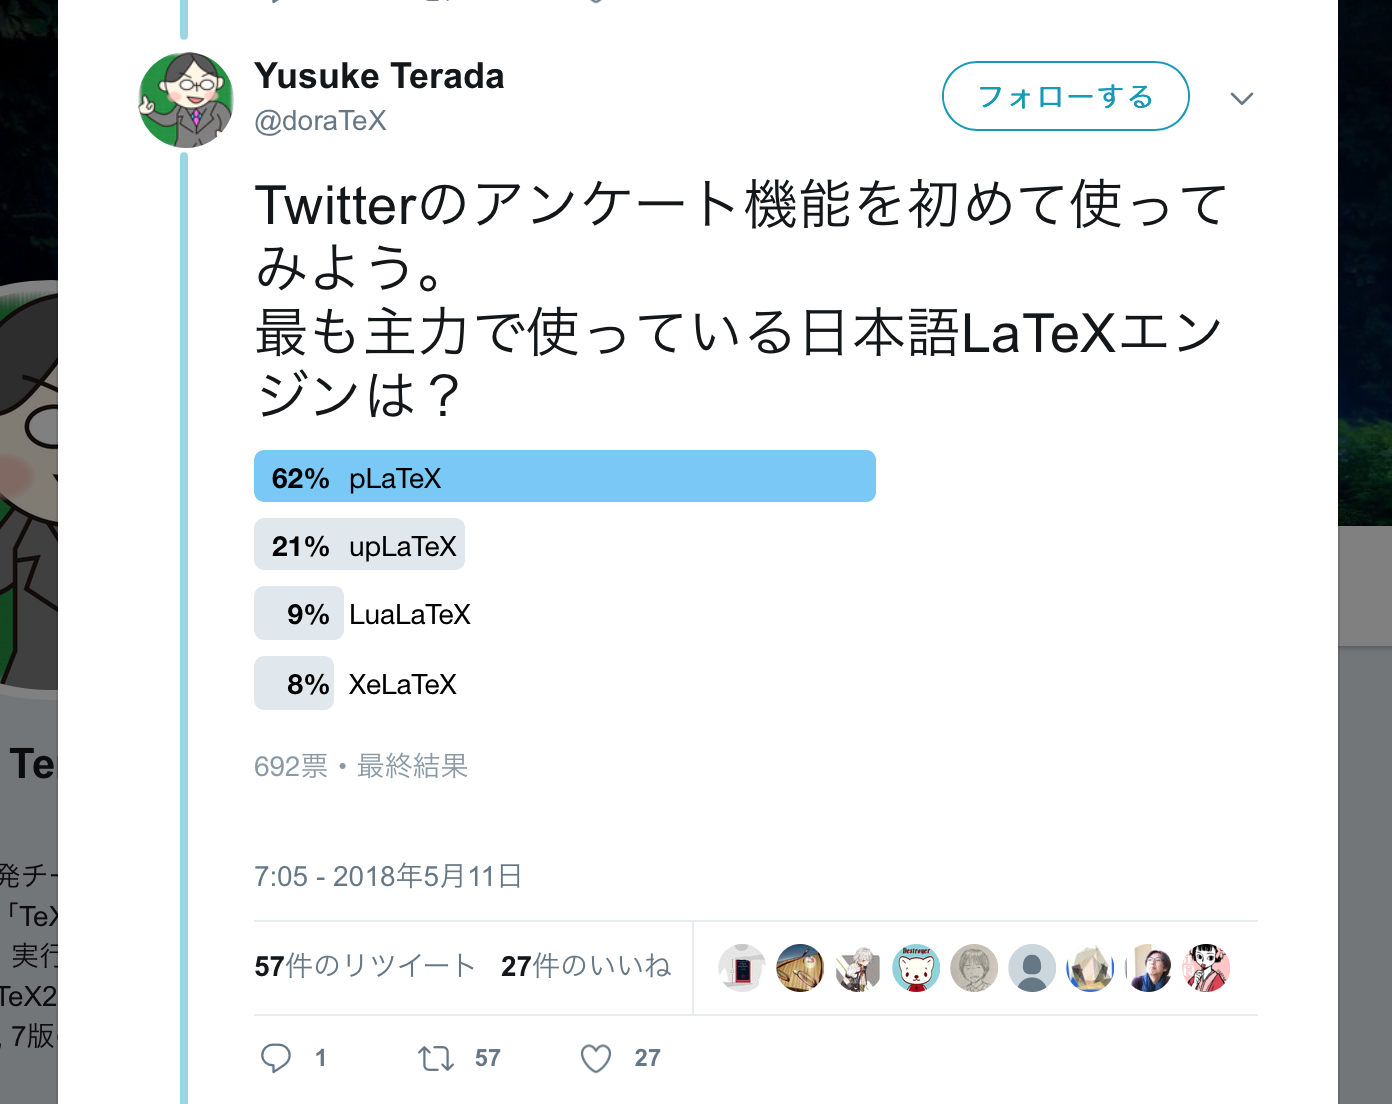
\includegraphics[width=\textwidth]{img/20180511-twitter-vote.png}%
  \par\vskip-7pt
  {\scriptsize\url{https://twitter.com/doraTeX/status/994941507730784257}}
\end{frame}

%% 4
\setbeamerfont{title}{family=,size=\large}
\setbeamerfont{author}{family=}
\setbeamerfont{date}{family=,size=\small}
\title{\pLaTeX ・\upLaTeX ユーザに贈る\\最新ベストプラクティス集}
\begin{frame}
  \maketitle
\end{frame}

%% toc (disabled for talk)
%\begin{frame}
%  \tableofcontents
%\end{frame}

%% 1-1
\Fsmile
\section{日本語の組版}
\subsection{モダンな\Lpack{jlreq}クラスを使おう}
\subsection{それ以外なら\Lpack{minijs}又は\Lpack{OTF}}
\frame{\sectionpage}

%% 1-2
\FsmileEX
\begin{frame}{\insertsectionnumber. \insertsection}
変なしがらみに悩まされる前に…
  \begin{itemize}
  \item モダンな\Lpack{jlreq}クラスを使おう\\[1ex]
  \pause
  \item \Lpack{beamer}などを使う場合\\[1ex]
        \TO \Lpack{minijs}あるいは\Lpack{OTF}を併用\\
    {\small\jfont\tradmin={SourceHanSans-Bold:jfm=min} at 14pt
     ({\tradmin ちょっと}変な詰まりから解放されます)}
  \end{itemize}
\end{frame}

%% 2-1
\Fsmile
\section{日本語フォント}
\subsection{まずは\Lpack{pxchfon}をチェック}
\frame{\sectionpage}

%% 2-2
\FsmileEX
\begin{frame}{\insertsectionnumber. \insertsection}
好きなフォントを使いたい…
  \begin{itemize}
  \item まずは\Lpack{pxchfon}をチェック\\
    {\small (比較的メジャー?\<なフォントなら簡単)}
  \end{itemize}
\pause
\medskip
使えるフォントを増やしたい…
  \begin{itemize}
  \item \cs{usepackage[deluxe]\{otf\}}\\
    {\small (フォントさえ揃えれば最大7書体化)}
  \end{itemize}
\end{frame}

%% 3-1
\Fsmile
\section{有力なパッケージの利用}
\subsection{とりあえず\Lpack{plautopatch}}
\frame{\sectionpage}

%% 3-2
\Ferror
\begin{frame}
  \centering
  \vfill
  {\LARGE \SUSHI これが意外と大変\SUSHI}
  \pause
  \par\vskip20pt
  …でした(ごく最近までは)
\end{frame}

%% 3-3(1)
\def\EXone{%
\item[\CRYING] とあるパッケージ
  %\footnote{\tiny \Lpack{ragged2e}, \Lpack{sidecap}, \Lpack{vwcol}など多種多様。}
  を読み込んだら
  \begin{itemize}
  \item OTFパッケージで文字化けしました
  \item ゴシック体になりません
  \item \cs{Large} などが効かなくなりました
  \end{itemize}
}
\FerrorEX
\begin{frame}{症例1(従来の対処法)}\small
\begin{description}
\EXone
\pause
\item[\TEACHER] もしこんな警告が出ていたら\\[1ex]
{\scriptsize \texttt{%
  ~LaTeX Warning: Command \cs{selectfont } has changed.\\
  ~~~~~~~~~~~~~~~~Check if current package is valid.}\par}
    …それは\Lpack{everysel}が原因で,\\
    \quad \underline{\Lpack{{\color{red}px}everysel}} を使えば解決します。
\end{description}
\end{frame}

%% 3-3(2)
\def\EXtwo{%
\item[\CRYING] \Lpack{plext}パッケージを読み込んだら\\[1ex]
  表(tabular環境)で謎のエラー\\[1ex]
{\footnotesize \texttt{%
  ! Missing \# inserted in alignment preamble.}}\\[1ex]
  が出ました
}
\FerrorEX
\begin{frame}{症例2(従来の対処法)}\small
\begin{description}
\EXtwo
\pause
\item[\TEACHER] 多分それは\Lpack{array}パッケージより{\color{red}後}に
  \Lpack{plext}パッケージを読み込んだからでしょう。\\[1ex]
  \Lpack{plext}は{\color{red}早めに} \cs{usepackage} しましょう。
  或いは,\underline{\Lpack{{\color{red}plext}array}} を代わりに使いましょう。
\end{description}
\end{frame}

%% 3-3(3)
\def\EXthree{%
\item[\CRYING] \Lpack{plext}パッケージと破線(\Lpack{arydshln}パッケージ)が
  同時に使えません\\[1ex]
{\scriptsize \texttt{%
  ! Undefined control sequence.\\[1ex]
  {\tiny
  \cs{adl@@cr} ...tempdima \cs{xdef} \cs{adl@rowsL} \{\cs{adl@rowsL} \\
  ~~~~~~~~~~~~~~~~~~~~~~~~~~~~~~~~~~~~~~~~~~~~~~~~~~(\cs{adl@colsL} ...}}\par}
}
\FerrorEX
\begin{frame}{症例3(従来の対処法)}\small
\begin{description}
\EXthree
\pause
\item[\TEACHER] \underline{\Lpack{{\color{red}plext}arydshln}} を使いましょう。
\end{description}
\end{frame}

%% 3-3(4)
\def\EXfour{%
\item[\CRYING] 縦書きで\TikZ を使おうとしたら\\[1ex]
{\scriptsize \texttt{%
  ! Incompatible direction list can't be unboxed.}}\\[1ex]
  が出ました
}
\FerrorEX
\begin{frame}{症例4(従来の対処法)}\small
\begin{description}
\EXfour
\pause
\item[\TEACHER] それは\Lpack{everyshi}パッケージが縦組非対応だからです。\\[1ex]
  \underline{\Lpack{{\color{red}px}everyshi}} を使いましょう。
\end{description}
\end{frame}

%% 3-3(5)
\def\EXfive{%
\item[\CRYING] 縦書きで\Lpack{atbegshi}を使おうとしたら\\やっぱり\\[1ex]
{\scriptsize \texttt{%
  ! Incompatible direction list can't be unboxed.}}\\[1ex]
  が出ました
}
\FerrorEX
\begin{frame}{症例5(従来の対処法)}\small
\begin{description}
\EXfive
\pause
\item[\TEACHER] それは\Lpack{atbegshi}パッケージが縦組非対応だからです。\\[1ex]
  \underline{\Lpack{{\color{red}px}atbegshi}} を使いましょう。
\end{description}
\end{frame}

%% 3-3(6)
\def\EXsix{%
\item[\CRYING] 縦書きで\Lpack{ftnright}を使おうとしたら\\やっぱり\\[1ex]
{\scriptsize \texttt{%
  ! Incompatible direction list can't be unboxed.}}\\[1ex]
  が出ました
}
\FerrorEX
\begin{frame}{症例6(従来の対処法)}\small
\begin{description}
\EXsix
\pause
\item[\TEACHER] それは\Lpack{ftnright}パッケージが縦組非対応だからです。\\[1ex]
  \underline{\Lpack{{\color{red}px}ftnright}} を使いましょう。
  ただし,これは\Lpack{ftnright}より{\color{red}前}に読み込む必要があります。
\end{description}
\end{frame}

%% 3-4
\def\oldsolution{%
{\scriptsize 左:\pLaTeX ・\upLaTeX でうまくいかないパッケージ,右:対策パッチ}\par
  \begin{itemize}\tiny
  \ITEMxTx  tracefnt  -> ptrace/uptrace
  \ITEMxTx  fltrace   -> pfltrace
  \ITEMxTx  array     -> plarray
  \ITEMxxTx array     +  plext  -> plextarray
  \ITEMxxTx delarray  +  plext  -> plextdelarray
  \ITEMxxTx colortbl  +  plext  -> plextcolortbl
  \ITEMxTx  arydshln  -> plarydshln
  \ITEMxxTx arydshln  +  plext  -> plextarydshln
  \ITEMxTx  siunitx   -> plsiunitx
  \ITEMxTx  everysel  -> pxeverysel (先に読んだ方が安全)
  \ITEMxTx  everyshi  -> pxeveryshi
  \ITEMxTx  atbegshi  -> pxatbegshi
  \ITEMxTx  ftnright  -> pxftnright (必ず先に読む)
  \ITEMxTx  pdfpages  -> pxpdfpages
  \ITEMxTx  pgfrcs  (\TikZ/PGF) -> pxpgfrcs
  \ITEMxTx  pgfcore (\TikZ/PGF) -> pxpgfmark
  \end{itemize}
\pause
\begin{description}\scriptsize
\item[\TEACHER] 左辺が別のパッケージによって \cs{RequirePackage} される場合も\\
  あります。同様に注意しましょう。
\end{description}}
\FerrorEX
\begin{frame}{まとめ(従来の対処法)}\relax
\oldsolution
\end{frame}

%% 3-5
\Ferror
\begin{frame}
  \centering
  \CRYING こんなの覚えられないよ\CRYING
\end{frame}

%% 3-6
\Fsmile
\begin{frame}
  \centering
  {\LARGE \LIGHTBULB そこで\LIGHTBULB}
\end{frame}

%% 3-7
\FsmileEX
\begin{frame}{作りました}
  \centering
  {\SCSNOWMAN\ \Lpack{plautopatch}パッケージ\ \SCSNOWMAN}
\end{frame}

%% 3-8
\FsmileEX
\begin{frame}{\Lpack{plautopatch}とは}\relax
\let\origpause\pause
\let\pause\relax
\oldsolution
\let\pause\origpause
\pause
\par\vskip-120pt
\rotatebox{15}{\PLAUTOPATCH}
\par\vskip120pt
\end{frame}

%% 3-9
\FsmileEX
\begin{frame}{\insertsectionnumber. \insertsection}
つまり\\[1ex]
\pLaTeX ・\upLaTeX で何かパッケージを使って変になったら\\
\TO とりあえずソースの{\color{red}冒頭}で\\
\qquad \cs{RequirePackage\{plautopatch\}}\\
してみましょう
\end{frame}

%% 3-10
\FsmileEX
\begin{frame}
  \centering
  {\Large\useKiloji\SCSNOWMAN\ めでたしめでたし\ \SCSNOWMAN}
\end{frame}

%% 3-11
\FsmileEX
\begin{frame}
  \centering
  {\LARGE \SCSNOWMAN\ おさらい\ \SCSNOWMAN}
\end{frame}

%% 3-11(1)
\FsmileEX
\begin{frame}{症例1(新対処法)}\small
\begin{description}
\EXone
\pause
\item[\TEACHER] \underline{\Lpack{{\color{red}plautopatch}}} を使いましょう
\end{description}
\end{frame}

%% 3-11(2)
\begin{frame}{症例2(新対処法)}\small
\begin{description}
\EXtwo
\pause
\item[\TEACHER] \underline{\Lpack{{\color{red}plautopatch}}} を使いましょう
\end{description}
\end{frame}

%% 3-11(3)
\begin{frame}{症例3(新対処法)}\small
\begin{description}
\EXthree
\pause
\item[\TEACHER] \underline{\Lpack{{\color{red}plautopatch}}} を使いましょう
\end{description}
\end{frame}

%% 3-11(4)
\begin{frame}{症例4(新対処法)}\small
\begin{description}
\EXfour
\pause
\item[\TEACHER] \underline{\Lpack{{\color{red}plautopatch}}} を使いましょう
\end{description}
\end{frame}

%% 3-11(5)
\begin{frame}{症例5(新対処法)}\small
\begin{description}
\EXfive
\pause
\item[\TEACHER] \underline{\Lpack{{\color{red}plautopatch}}} を使いましょう
\end{description}
\end{frame}

%% 3-11(6)
\begin{frame}{症例6(新対処法)}\small
\begin{description}
\EXsix
\pause
\item[\TEACHER] \underline{\Lpack{{\color{red}plautopatch}}} を使いましょう
\end{description}
\end{frame}

%% 4-1
\FsmileEX
\begin{frame}{今日のまとめ}
  \tableofcontents
\end{frame}

%% 4-2
\FsmileEX
\begin{frame}
  \centering
  {\LARGE\useKiloji\SCSNOWMAN\ おしまい\ \SCSNOWMAN}
\end{frame}

\end{document}
